\documentclass{article}
\usepackage{listings}
\usepackage[margin=1in]{geometry}
\usepackage{graphicx}
\usepackage{amsmath}
\usepackage[ruled,vlined]{algorithm2e}


\title{CMOR 421/521, Homework \#4: \LaTeX{} Submission}
\author{\texttt{amc50}}
\date{April 28, 2024}

\begin{document}

\maketitle

\section{Compilation}

All procedures and results discussed were conducted on the NOTS Cluster. To replicate these results, access to a GPU-enabled node on the NOTS cluster is essential. This can be efficiently achieved by utilizing the \texttt{CMOR 421} reservation.

\bigskip
\noindent
Command used to acquire a GPU-enabled node on NOTS:

\begin{verbatim}
[amc50@nlogin1 homework-4]$ srun --pty --partition=scavenge
--reservation=cmor421 --ntasks=1 --mem=1G --gres=gpu:1 --time=04:00:00 $SHELL
\end{verbatim}

\bigskip
\noindent
Accessing the NVIDIA Profiler, \texttt{nvprof}, requires loading specific modules in a precise sequence. The commands for managing these modules are as follows:

\bigskip
\noindent
Command used to clear all previously loaded modules:

\begin{verbatim}
[amc50@bc8u27n1 homework-4]$ ml purge
\end{verbatim}

\bigskip
\noindent
Command used to load the necessary module for compilation:

\begin{verbatim}
[amc50@bc8u27n1 homework-4]$ ml load GCC/8.3.0
\end{verbatim}

\bigskip
\noindent
Command to load the CUDA module, which provides access to \texttt{nvprof}:

\begin{verbatim}
[amc50@bc8u27n1 homework-4]$ ml load CUDA/10.1.168 
\end{verbatim}

\bigskip
\noindent
To compile CUDA files, the \texttt{nvcc} compiler is used. The version variable \(\$vi\) is introduced in this compilation discussion to denote different versions of both the reduction and stencil implementations that utilize the same sequence of compilation commands.

\bigskip
\noindent
For each version \(i = 0, 1, 2\), the command to compile the reduction implementations is:

\begin{verbatim}
[amc50@bc8u27n1 homework-4]$ nvcc reduction_$vi.cu -o $vi
\end{verbatim}

\bigskip
\noindent
For each version \(i = 0, 1, 2\), the command to profile and run reduction implementations is:

\begin{verbatim}
[amc50@bc8u27n1 homework-4]$ nvprof ./reduction_$vi
\end{verbatim}

\bigskip
\noindent
This process is similarly repeated for the stencil implementations, with the addition that the stencil executable requires a block size. For this example, a block size of \(b = 128\) is used.

\bigskip
\noindent
For each version \(i = 1, 2\), the command to compile stencil implementations is:

\begin{verbatim}
[amc50@bc8u27n1 homework-4]$ nvcc stencil_$vi.cu -o stencil_$vi
\end{verbatim}

\bigskip
\noindent
For each version \(i = 1, 2\), the command to profile and run stencil implementations with a block size of 128 is:

\begin{verbatim}
[amc50@bc8u27n1 homework-4]$ nvprof ./stencil_$vi 128
\end{verbatim}

\bigskip
\noindent
To generate timings for various implementations, Bash scripts were created, utilizing different metrics from \texttt{nvprof}. These scripts facilitate the generation of kernel timings and the determination of floating-point operations. For the stencil implementations, the block size varies as \(b = 2^i\) for \(i = 1, \ldots, 10\). Separate timing scripts for the two stencil versions were created to simplify post-processing.

\bigskip
\noindent
Command to generate timings for the reduction implementations:
\begin{verbatim}
[amc50@bc8u27n1 homework-4]$ ./generate_reduction_timings.sh 
\end{verbatim}

\bigskip
\noindent
Command to generate timings for stencil version 1 implementation:
\begin{verbatim}
[amc50@bc8u27n1 homework-4]$ ./generate_stencil_v1_timings.sh 
\end{verbatim}

\bigskip
\noindent
Command to generate timings for stencil version 2 implementation:
\begin{verbatim}
[amc50@bc8u27n1 homework-4]$ ./generate_stencil_v2_timings.sh 
\end{verbatim}

\section{Reduction Implementation}

\subsection{Reduction Timings}
\begin{table}[ht!]
    \caption{Reduction Timings on NOTS}
    \centering
    \begin{tabular}{|c|c|c|}
        \hline
         & Time (Milliseconds) & Floating Point Operations  \\
        \hline
        Version 0 & 1.317 & 4161536 \\
        \hline
        Version 1 & 0.824 & 4161536 \\
        \hline
        Version 2 & 0.415 & 4177920 \\
        \hline
    \end{tabular}
\end{table}

\subsection{Reduction Version 0}

There is a marked difference in performance between Version 0 and Version 1 of the reduction algorithm. Both versions are nearly identically, using a logarithmically decreasing number of threads, equivalent memory accesses, and same number of arithmetic operations. As such, the difference must result from their distinct communication patterns. For Version 0, the alive threads are determined by progressively increasing the stride with each iteration. Version 1, instead, has the upper half of live threads send the information to the lower half of live threads. Given the GPU's hardware limitations, each warp, typically 32 threads, executes the same instruction all together. This structure thus requires the execution of both branches of any conditional. As the stride grows for version 0, then it increases this divergence within a warp, leading to a higher number of idle threads. Comparatively, Version 1 limits the branch divergence by keeping the active threads in contiguous positions. This alignment aids in having all threads in a warp execute the same instruction, which reduces the inefficiencies in Version 0 and results in the observed improved runtime. 

\subsection{Reduction Version 2}
Reduction Version 2 significantly enhances performance, nearly halving the runtime compared to Version 1. This improvement stems from the strategic modifications in Version 2's thread management and data handling. Both versions follow an identical approach for deactivating threads, sending information from the upper half of the alive threads to the lower half. However, Version 2 improves performance by having each thread initially sum two elements from global memory before storing the result in shared memory. This adjustment ensures that all threads are actively participating, minimizing idle time. Additionally, while this requires additional computation for each thread at the start, it substantially reduces the thread overhead, decreasing the total number of thread blocks by half. This structure also requires that each thread still performs coalesced memory reads from global memory when accessing the two elements. If this was not the case, the observed performance gains would not be observed.

\subsection{Roofline Plot Results}

For the following roofline plots, the reduction implementations were executed on the NOTS Cluster, which is equipped with a NVIDIA Tesla K80 GPU. This GPU has a maximum aggregate memory bandwidth of 480 GB/s with up to 4.113 TFLOPS/s for single-precision performance. The theoretical upper bound of the roofline is calculated as the minimum between the peak performance and the product of computational intensity, \(CI\), and peak bandwidth. Each data point on the roofline plot represents the operational intensity in FLOPS/byte versus the achieved performance in GFLOPS/s.

\bigskip
\noindent
To determine the operational intensity, \(CI\) must be calculated and is defined as the average number of floating-point operations (flops) per slow memory access, denoted \(\frac{f}{m}\). For the zeroth and first version of the reduction algorithm, the number of arithmetic operations \( f \) is calculated as \( f = n - \frac{n}{b} \), where \( n \) is the size of the vector and \( b \) is the block size. In this case, \( n = 2^{22} \) and \( b = 128 \), resulting in an expected \( 2^{22} - \frac{2^{22}}{128} = 4,161,536 \) flops. This calculation is verified using the \texttt{nvprof} metric \texttt{flop\_count\_sp}. Furthermore, the number of slow memory accesses, \( m \), is given by \( m = n + \frac{n}{b} \). Currently, to the best of my knowledge there is no direct metric in \texttt{nvprof} that provides the memory access count in the same straightforward manner as it does for flop counts. For the second version of the reduction algorithm, \( f = n - \frac{n}{2 \cdot b} \) and \( m = n + \frac{n}{2 \cdot b} \). As before, this calculation is verified using \texttt{nvprof}, confirming the flop count as 4,177,920. The resulting computational intensity for the zeroth and first version is given by equation (1) and for the second version by equation (2). It is important to note that, unlike previous calculations of computational intensity necessitating division by 8 for conversion into units of 64-bit double-precision words, these calculations for single-precision operations involve division by 4, corresponding to the 32-bit word size. 

\begin{equation}
CI = \frac{n + \frac{n}{b}}{(n - \frac{n}{b}) \times 4}
\end{equation}

\begin{equation}
CI = \frac{n + \frac{n}{2 \cdot b}}{(n - \frac{n}{2 \cdot b}) \times 4}
\end{equation}

\bigskip
\noindent
At this point, all required information is determined and the roofline plot can be generated. The resulting plot can be seen in Figure 1.

\clearpage

\begin{figure}[!htb]
    \centering
    \fbox{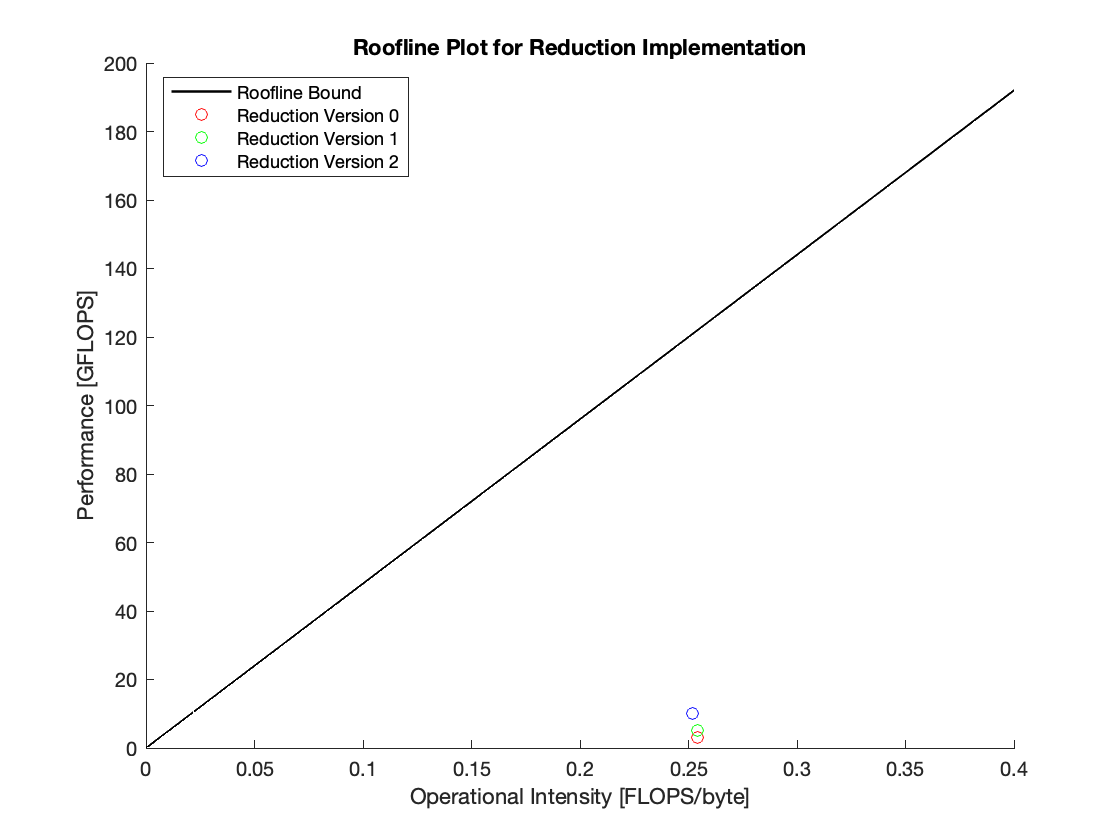
\includegraphics[width=0.8\linewidth]{reduction_roofline.png}}
    \caption{Roofline Plot for Reduction Implementations}
\end{figure}

\section{Stencil Implementation}

\subsection{Stencil Version 1}

Stencil Version 1 implements the stencil computation described in equation (3), utilizing global memory for data access. In the context of this equation, we set $\alpha = 1$, and address boundary conditions with $x_0$ and $x_{n+1}$. Managing these global boundary conditions is critical in this implementation. While a straightforward approach might involve conditional statements to check if an element is at the beginning or end of the vector, it is crucial to avoid branching where possible to optimize performance. Therefore, ternary operators are employed to reduce divergence within a warp.

\bigskip
\noindent
To verify the correctness of this implementation, all elements, $x_i$, are initialized to 1, given that it is expected the the stencil operation results in $y_i = 0$. The correctness is further ensured by using the \texttt{flop\_count\_dp} metric to confirm that all computations are performed using single precision. The timing results for varying block sizes are presented in Table 2.

\begin{gather}
    y_i = \alpha (-x_{i+1} + 2x_i - x_{i-1}) \nonumber \\
    x_0 = x_1 \nonumber \\
    x_{n+1} = x_n
\end{gather}

\clearpage

\begin{table}[ht!]
    \caption{Stencil Version 1 Timings on NOTS}
    \centering
    \begin{tabular}{|c|c|}
        \hline
        Block Size & Time (Milliseconds) \\
        \hline
        b = 2 & 15.458\\
        \hline
        b = 4 & 7.7494\\
        \hline
        b = 8 & 3.9018\\
        \hline
        b = 16 & 1.9925\\
        \hline
        b = 32 & 1.0145\\
        \hline
        b = 64 & 0.557\\
        \hline
        b = 128 & 0.328\\
        \hline
        b = 256 & 0.339\\
        \hline
        b = 512 & 0.358\\
        \hline
        b = 1024 & 0.406\\
        \hline
    \end{tabular}
\end{table}

\subsection{Stencil Version 2}

Stencil Version 2 advances the computation of the stencil described in equation (3) by leveraging shared memory. As before, to confirm the implementation all elements are set to $x_i = 1$, and it is checked that all operations were single-precision. A key distinction of Version 2 lies in the optimization of the block size, which is crucial given that the shared memory is allocated to be \texttt{BLOCK\_SIZE} + 2 additional elements to account for halo cells. As seen in Table 3, the optimal block size was found to be $b = 128$, which matches the best-performing block size identified in Version 1's timing results. This consistency suggests that the optimal block size is influenced by the hardware architecture, as it represents an integer multiple of the warp size, which is commonly 32 threads. For this case then that multiple is 4.

\bigskip
\noindent
This shared memory strategy requires dividing the global data array into segments, each sized \texttt{BLOCK\_SIZE} + 2 to include halo cells. Halo cells allow the stencil to separate out arrays while still giving edge points access to the adjacent cells necessary to complete the stencil operation. If this was not the case, the points would be outside the available scope and would block the implementation. Indexing within the shared memory also introduces additional complications. Unlike the straightforward global indexing of Version 1, shared memory indexing must account for the halo cells and local thread ids. Part of this challenge is filling the local arrays with the global information. For this process, as before, ternary operators were used when possible. However, due to the complexity if-else statements were used although there is likely an approach that avoids these entirely. 

\begin{table}[ht!]
    \caption{Stencil Version 2 Timings on NOTS}
    \centering
    \begin{tabular}{|c|c|}
        \hline
        Block Size & Time (Milliseconds) \\
        \hline
        b = 2 & 20.743\\
        \hline
        b = 4 & 10.389\\
        \hline
        b = 8 & 5.1991\\
        \hline
        b = 16 & 2.6136\\
        \hline
        b = 32 & 1.3150\\
        \hline
        b = 64 & 0.694\\
        \hline
        b = 128 & 0.402\\
        \hline
        b = 256 & 0.407\\
        \hline
        b = 512 & 0.428\\
        \hline
        b = 1024 & 0.485\\
        \hline
    \end{tabular}
\end{table}

\subsection{Roofline Plot Results}

As discussed above, the roofline plot necessitates the calculation of the computational intensity \(CI\). The method previously described, which involves determining the number of arithmetic operations \(f\), verifying with \texttt{nvprof}, and calculating the theoretical number of slow memory accesses, will be employed again here. For Stencil Version 1, the number of arithmetic operations, \(f\), is \(3 \times n\). For this implementation a vector of size \(n = 2^{22}\) is used, resulting in 12,582,912 single precision floating-point operations. The number of memory accesses, \(m\), is \(4 \times n\), accounting for 3 reads from global memory and 1 write. The resulting computational intensity is given by equation (4):

\begin{equation}
    CI = \frac{3 \cdot n}{4 \cdot n \cdot 4} = \frac{3}{16}
\end{equation}

\bigskip
\noindent
Similarly, for Stencil Version 2, the number of arithmetic operations remains \(f = 3 \times n\). However, the number of global memory accesses differs; there is one load from global to shared memory and one write, making \(m = 2 \times n\). In reality, it will be slightly larger due to the halo loading, but for the purposes of this study these are negligible in comparison to $n$. The computational intensity for this version is given by equation (5):

\begin{equation}
    CI = \frac{3 \cdot n}{2 \cdot n \cdot 4} = \frac{3}{8}
\end{equation}

\noindent
These calculations are then applied to the roofline plot, as shown in Figure 2.

\begin{figure}[!htb]
    \centering
    \fbox{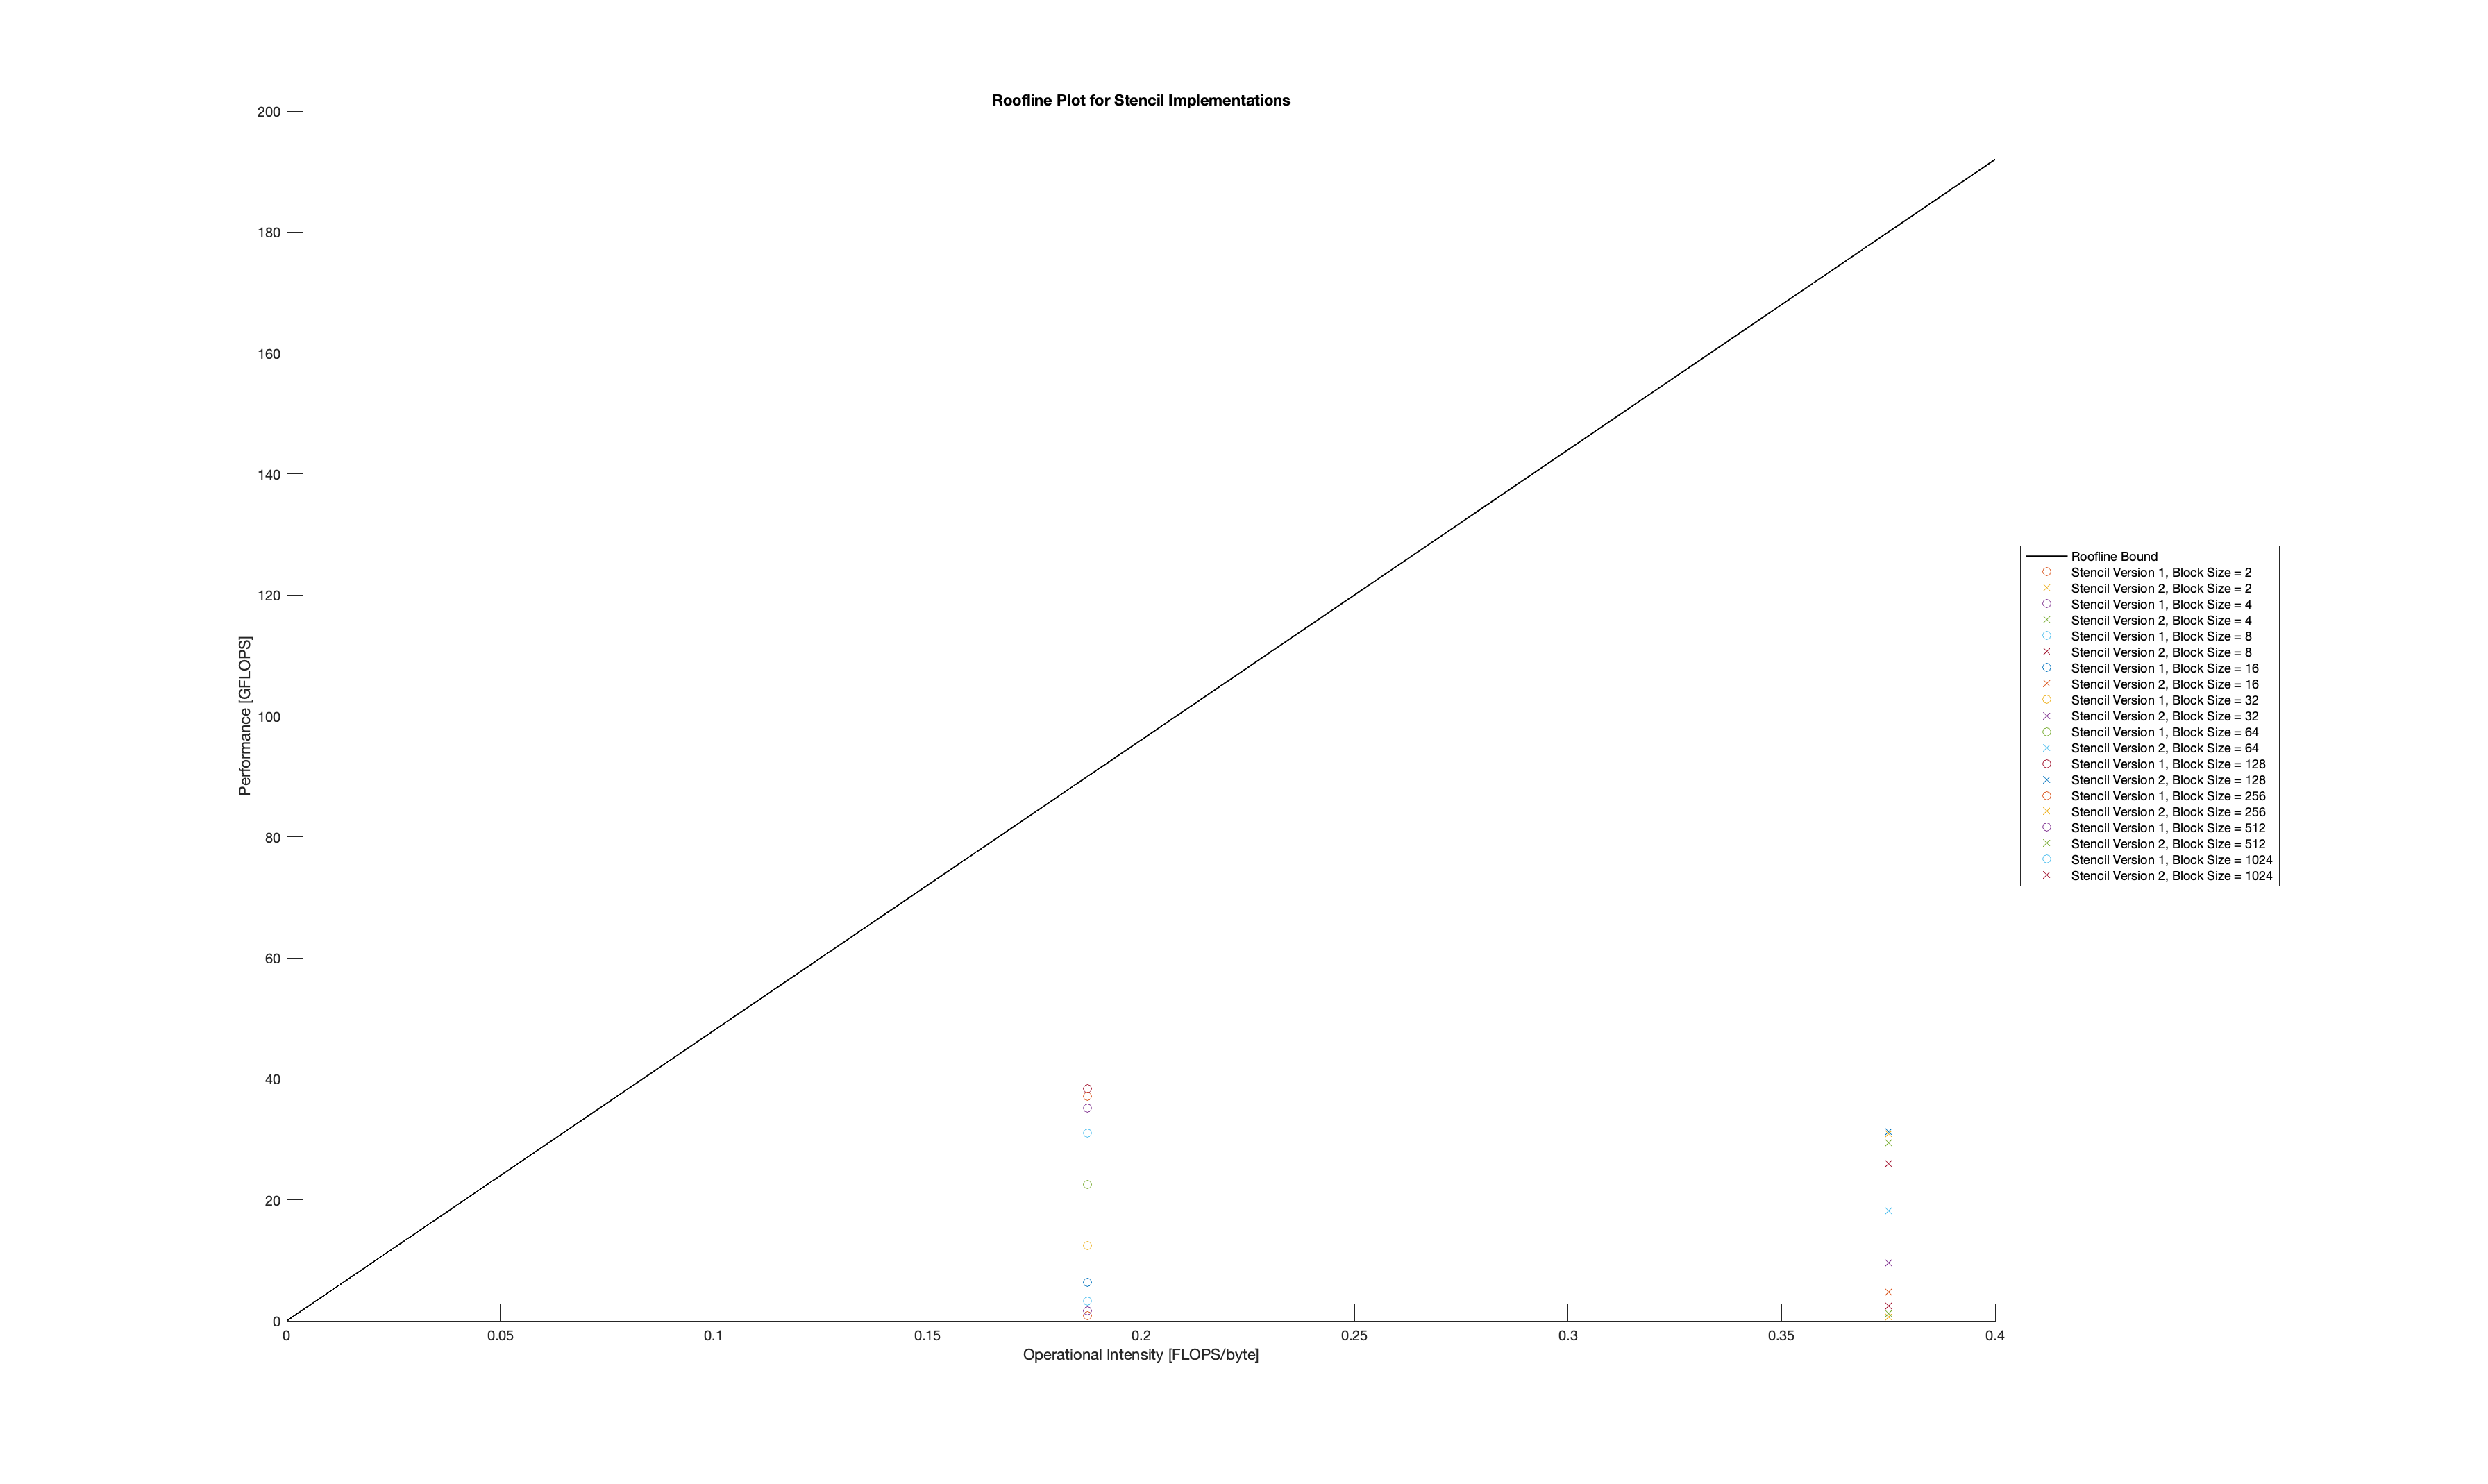
\includegraphics[width=0.8\linewidth]{stencil_roofline.png}}
    \caption{Roofline Plot for Stencil Implementations}
\end{figure}

\section{Roofline Plot Analysis}

Interestingly, Version 2 did not outperform Version 1. For smaller block sizes, Version 2 demonstrated notably slower execution times, and even at the optimal block size, Version 1 maintained a slight lead. As previously discussed, the computational intensity for Version 2 is twice that of Version 1, leading to the expectation that Version 2 should exhibit enhanced performance since a higher CI typically correlates with reduced execution time. The observed under performance is then likely resulting from the implementation details rather than the actual implementation algorithm. Specifically, the incorporation of dual if-else statements introduces branching to manage edge cases, consequently incurring a performance penalty. It is important to note that at the optimal block size, Version 1 approaches over 50\% of the theoretical peak performance as defined by the roofline model. Although the peak performance is very low at this computational intensity, it is still superior to the performance of Version 2. These findings suggest that while computational intensity is a significant factor, other aspects such as branching and memory access patterns play a pivotal role in determining overall performance. 
\end{document}
